\documentclass[acmlarge]{acmart}

\usepackage{booktabs} % For formal tables
\usepackage{xxxnotes} 
\usepackage{upgreek} 
\usepackage{tikz}
\newtheorem{theorem}{Theorem}

\newenvironment{proof-sketch}{%
      \renewcommand{\proofname}{Proof Sketch}\proof}{\endproof}
% Metadata Information
%\acmJournal{PACMHCI}
%\acmVolume{9}
%\acmNumber{4}
%\acmArticle{39}
%\acmYear{2010}
%\acmMonth{3}
%\acmArticleSeq{11}

%\acmBadgeR[http://ctuning.org/ae/ppopp2016.html]{ae-logo}
%\acmBadgeL[http://ctuning.org/ae/ppopp2016.html]{ae-logo}


% Copyright
%\setcopyright{acmcopyright}
%\setcopyright{acmlicensed}
%\setcopyright{rightsretained}
%\setcopyright{usgov}
%\setcopyright{usgovmixed}
%\setcopyright{cagov}
%\setcopyright{cagovmixed}

% DOI
%\acmDOI{0000001.0000001}

% Paper history
%\received{February 2007}
%\received{March 2009}
%\received[accepted]{June 2009}


% Document starts
\begin{document}
% Title portion
\title{The Price of Human Nature}

\author{Lillian Tsai}
\orcid{1234-5678-9012-3456}
\affiliation{%
  \institution{MIT}
  \city{Cambridge}
  \state{MA}
  \country{USA}}
\email{tslilyai@mit.edu}
\author{Vibhaalakshmi Sivaraman}
\affiliation{%
  \institution{MIT}
  \city{Cambridge}
  \state{MA}
  \country{USA}}
\email{vibhaa@mit.edu}
\author{Xiaoyue Gong}
\affiliation{%
  \institution{MIT}
  \city{Cambridge}
  \state{MA}
  \country{USA}}
\email{xygong@mit.edu}

%\begin{abstract}
%The impact of selfish actions on the latency incurred by a network users has historically been a problem of great interest to the algorithmic community. Our paper first presents a brief overview of the original selfish routing problem, the standard algorithms used to route in the selfish routing setting, and the limits on the optimality of these algorithms (termed as the ``price of anarchy"), and then compare and contrasts other recent works that have formulated the problem in
%    (perhaps more realistic) settings, i.e., by taking into account the possibility for altruistic, risk averse, and diverse-interest behaviors.  This paper both presents and clarifies the findings of these papers in the context of the original selfish routing paper, and demonstrates how these papers' results can be synthesized into a more general framework addressing optimality of routing with various human behaviors or motivations.
%\end{abstract}

%\keywords{selfish routing, price of anarchy}

\maketitle

\section{Introduction}
Finding the best strategy for network and traffic routing has historically been a problem of great importance combining the theoretical aspects of both game theory and computer science. 
\begin{itemize}
    \item Introduce noncooperative games / Nash equilibrium (in network setting)
    \item Briefly introduce selfish routing paper / price of anarchy
    \item Discuss how it is a limited view of human behavior
    \item Briefly discuss alternatives (papers including taxes, different objectives, atomic games, studies on network structure)
    \item Us: There are newer papers with more interesting versions of human behavior, and we present a survey of these newer papers to show how human behaviors affect price of anarchy
\end{itemize}

\section{Background}
\label{sec:background}
This section presents a brief history of traffic routing problem and the selfish routing model, defining the terminology and context in which 
we describe later results.

\subsection{The Traffic Routing Problem}
Traffic routing problems naturally arise in communication or transportation networks, where users are trying to minimize the latency that they or their data experiences.
However, links in the network often become \emph{congested} if too many users decide to route their data 
or cars through that link. Consequently, in these networks, the path each user chooses can affect the travel times of other
users. Here, we describe Roughgarden and Tardos' formalization of the problem of minimizing latency as multicommodity flow networks~\cite{tardos,roughgarden}, and use Pigou's example network in Figure~\ref{fig:Pigou} as a running example. We will later use this to reason about how much latency increases from optimum when users make selfish routing decisions.

\begin{figure}[ht!]
\begin{center}
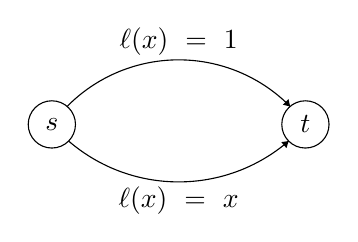
\begin{tikzpicture}[scale=0.1]
\tikzstyle{every node}+=[inner sep=0pt]
\draw [black] (18,-17.9) circle (3);
\draw (18,-17.9) node {$s$};
\draw [black] (50.2,-17.9) circle (3);
\draw (50.2,-17.9) node {$t$};
\draw [black] (19.94,-15.615) arc (135.3471:44.6529:19.905);
\fill [black] (48.26,-15.62) -- (48.05,-14.69) -- (47.34,-15.4);
\draw (34.1,-9.2) node [above] {$\ell(x)\mbox{ }=\mbox{ }1$};
\draw [black] (48.072,-20.011) arc (-49.23907:-130.76093:21.4);
\fill [black] (48.07,-20.01) -- (47.14,-20.15) -- (47.79,-20.91);
\draw (34.1,-25.7) node [below] {$\ell(x)\mbox{ }=\mbox{ }x$};
\end{tikzpicture}
\end{center}
    \caption{Pigou's example traffic routing problem, with a demand of $r_{(s,t)} = 1$}
\label{fig:Pigou}
\end{figure}

\medskip\noindent
\textbf{The input} $(G,r,\ell)$ to a traffic routing problem consists of:
\begin{itemize}
    \item A network $G = (V, E)$ of $|V|$ destinations (e.g., locations or servers) and $|E|$ links 
     \item A set of $k$ source-destination pairs $S=\{(s_1,t_1), \cdots (s_k,t_k)\}$ representing traffic demands
    \item A {rate} $r_i$ of traffic for each $(s_i,t_i)\in S$ representing the demanded amount of traffic from $s_i$ to $t_i$
    \item A {latency} function $\ell$ that assigns a per-edge function $\ell_e$ to each edge $e$ describing how adding traffic (i.e., congestion) to $e$ affects the time taken to travel across $e$. We can also think of $\ell$ as assigning per-path latencies: for any path $p$ in the graph
        $$\ell_p(f) = \sum_{e\in P}\ell_e(f_e)$$ 
        We assume that $\ell$ is continuous, nonnegative, and nondecreasing.
\end{itemize}
In Figure~\ref{fig:Pigou}, we see a single source-destination input network with an example (linear) cost function with $r_{(s,t)} = 1$.

\medskip\noindent
\textbf{Solutions} correspond to flow assignments to the set of simple paths $P_i$ between $s_i$ and $t_i$ for all $i$. Note that our solutions assume \emph{nonatomic} entities: the flows we find may not be integral.
Intuitively, this means that the demand from one $s_i$ to $t_i$ is generated by an infinite number
of entities in the network, which allows us to reason about continuous, rather than discrete, functions.
%
We can describe a flow assignment $f$ via use its path decomposition ($f$ is made up of flows $f_p$, the flow on a single path $p \in P_i$, where $f_p$ flow is added to all edges in $p$); alternatively, we can describe the flow on each edge $f_e = \sum_p \sum_{e\in p} f_p$, (equal to the sum of flow on all paths that use $e$).

A \emph{feasible} solution given such an input is an assignment of path flows such that the demand from $s_i$ to $t_i$ is met:
$$\forall 1 \le i \le k,~\sum_{p\in P_i} f_p = r_i$$
%
An \emph{optimal} (feasible) solution given such an input is the feasible flow assignment $f$ that minimizes the \textbf{social welfare latency cost} $C(f)$, where
$$C(f) = \sum_i\sum_{p\in P_i}\ell_p(f)f_p = \sum_{e\in E} f_e\ell_e(f_e)$$

Intuitively, we are calculating the latency of each path of a given flow assignment, weighing 
each path's latency proportional to the amount of flow through the path. More concretely,
if we were to let flow represent the routes chosen by (infinitely many) users, $C(f)$ calculates the average latency over all users. Thus, when minimizing $C(f)$, some users may incur 
more latency so that other users can go faster: the optimal flow is the \emph{socially optimal} solution.
Note that there exists an optimal flow $f^*$ minimizing $C(f)$ because we assume $\ell$ is continuous and the set of feasible flows is compact.

In our running example (Figure~\ref{fig:Pigou}), a feasible flow is any flow that sends one unit from $s$ to $t$ (divided in any fashion between the top and bottom edges).
The optimal flow is the flow that sends half the traffic through the lower edge and half through the upper edge: the users on the lower edge only experience a latency of $1/2$, while the users on the upper edge experience a latency of $1$, making the social welfare cost cost $3/4$.

\subsection{Coordination Models and the Price of Anarchy}
Before we can create algorithms to solve the traffic routing problem, we must first assume a \emph{coordination model} for our traffic network.
There are two clear extremes: (1) centralized control, in which some entity (e.g., an air traffic controller) knows all traffic demands and routes accordingly, and
(2) decentralization, i.e., a complete \emph{lack} of coordination between
entities in the network.
In a centralized setting, there is a clear optimal solution, as shown in the previous section.
However, in a decentralized and uncoordinated model, the lack of coordination and the exercise of free will can result in
inefficiencies. 

\medskip
\textbf{The Price of Anarchy} (PoA) allows us to measure the inefficiencies of a decentralized model, and was first introduced by Koutsoupias and Papadimitriou in 1999~\cite{poa}. 
We treat the decentralized model as a game in which each individual optimizes for her own \textbf{individual cost function $c$}, allowing us to compute the achieved flow at the resulting Nash equilibrium (proven to exist if the cost functions are continuous)~\cite{wardrop,haurie,beckmann1956studies}.
The price of anarchy $\rho(G,r,\ell)$ is defined as the ratio between the optimally minimal social welfare latency cost, and the social welfare latency cost at the flow achieved at Nash equilibrium.
(This is similar to how we measured the distance from optimal of an approximation algorithm in a limited computational power model, and of online algorithms in an incomplete information model.)

The set of flows at Nash equilibrium are defined such that for all $i$ source-destination pairs, all the paths from $s_i \to t_i$ have the minimum-possible cost with respect to an individual's cost function $c$. In other words, the (nonzero) flow paths at Nash equilibrium have equal path costs, and no user decreases her cost by choosing a different path:
$$\forall 0\le i \le k,~\forall p_1, p_2\in P_i~s.t.~f_{p_1} > 0~\text{and} f_{p_2} > 0,~ c_{p_1}(f) = c_{p_2}(f)$$
Note that this corresponds exactly to the solutions to the following (convex) program solvable in polynomial time:
$$NE = \min_f\Big(\sum_e \int_0^{f_e} c_e(t)dt\Big) \text{ subject to feasibility constraints}$$
whereas the flow optimizing the social welfare latency cost corresponds exactly to the (polynomial-time) solutions to the following (convex) program: 
$$SW = \min_f\Big(\sum_e f_e\ell_e(f_e)\Big) \text{ subject to feasibility constraints}$$

\subsection{The Selfish Routing Model}
One example of an uncoordinated model is the \emph{selfish routing} model, in which all entities in the network are selfish and choose a route minimizing their individual latency without caring (or knowing) about the effects on other users~\cite{tardos}.
The selfish routing model corresponds to flows at a Nash equilibrium where each user optimizes her individual cost function
$c^s(f) = l(f)$.
Thus, the program optimized at Nash equilibruim is
$$NE^{s} = \min_f\Big(\sum_e \int_0^{f_e} \ell_e(t)dt\Big) \text{ subject to feasibility constraints}$$

If we revisit our running example in Figure~\ref{fig:Pigou}, we note that the flow at Nash equilibrium corresponds to a flow that sends the entire unit of traffic through the bottom edge (the 0 flow through the top path has latency 1, and the unit flow through the bottom path will have latency 1).
Intuitively, each user routing from $s$ to $t$ will selfishly choose to take the bottom route because she will reason that the bottom route can have latency no worse than the top route. However, by doing so, the bottom route becomes more congested and leads to a total average latency $C(f) = 1$.
Thus, in Figure~\ref{fig:Pigou}, the price of anarchy $\rho$ is $\frac{1}{3/4} = \frac{4}{3}$.

We next describe and present the main results regarding the price of anarchy in this (decentralized) selfish routing model, which will act as a basis to which we will compare traffic routing results in more recently formulated models.

\subsection{Main Results}
\begin{theorem}
    If $f$ is a flow at Nash equlibrium for a given input set $(G, r, \ell)$ and $f^*$ is a feasible flow for $(G, 2r, \ell)$, then $C(f) \leq C(f^*)$
\end{theorem}

\begin{proof-sketch}
    This result demonstrates that the latency incurred when users selfishly route $r$ units of flow is at most the optimal (minimum) latency routing twice as much demand ($2r$).

\begin{figure}[t!]
    \centering
    \includegraphics[width=.7\textwidth]{graph}
    \caption{Visualizing latency costs of individual edges}
    \label{fig:thm1}
\end{figure}

    For any Nash equilibrium solution $f$ for $(G, r, \ell)$ and any feasible solution $f^*$, we can draw a figure like Figure~\ref{fig:thm1} for each edge $e$ in $G$, where $A,~B,~C,~D,\text{ and } E$ represent the magnitude of the areas of the indicated portions of the graph.
    $A+B$ represents the latency cost $C(f)$ of the Nash equilibrium solution $f$ for $(G, r, \ell)$, and $B+C$ represents the cost $C(f^*)$ of the feasible solution $f^*$ for $(G, 2r, \ell)$. 
    
    Since $D+E \le D+B+C$, and $D < A+B$, we know that $D+E-(B+C)\le D \le A+B $. This means that $B+C\ge D+E -(A+B)$. On the other hand $D+E\ge 2(A+B)$. Therefore, we have that $C(f^*)=(B+C)\ge 2(A+B)-(A+B)= A+B= C(f)$. 
    This indicates that the latency of any Nash equilibrium flow for $(G, r, \ell)$ is no bigger than represents the latency of any feasible solution for $(G, 2r, \ell)$.
    
    The main idea of the proof for this theorem lies in that the subset if the area $C$ is at least as big as the area $A+B$. This is always true because the latency $\bar{\ell}_e$ is a nondecreasing function and thus the graph of latency function gives a shape that looks like a generalized trapezoid (in particular, a right generalized trapezoid lying on the horizontal axis). 
    %Then we can obtain the result based on the property of a trapezoid shape. Therefore, the cost of any feasible solution for $(G, 2r, \ell)$ is at least twice the cost $C(f)$ of any Nash equilibrium solution for $(G, r, \ell)$. Then the area under the black line from $0$ to $2f_e$ in subgraph (a) is at least $2C(f)-C(f)$ and thus larger than $C(f)$. 
   %The cost of any feasible solution for $(G, 2r, \ell)$, and the area under the black line from $0$ to $2f_e$ in subgraph (b) is at most $C(f)$ more than the cost of any feasible solution for $(G, 2r, \ell)$, and the area under the black line from $0$ to $2f_e$ in subgraph (a). So the area of the generalized trapezoid under the black line from $0$ to $2f_e$ is more than two times the area under the black line on the left side of $f_e$ in subgraph (b). 
    %$+E$ under the black line from $0$ to $2f_e$ in subgraph (b) represents the cost of any feasible solution for $(G, 2r, \ell)$. The area under the black line on the left side of $f_e$ in subgraph (a) represents the cost $C(f)$ of any Nash equilibrium solution for $(G, r, \ell)$. Note that since the area of t he area under the black line on the left side of $f_e$ in subgraph (a) is at least half of the dashed line, we know that the cost of any feasible solution for $(G, 2r, \ell)$, and the area under the black line from $0$ to $2f_e$ in subgraph (b) is at most $C(f)$ more than the cost of any feasible solution for $(G, 2r, \ell)$, and the area under the black line from $0$ to $2f_e$ in subgraph (a). So the area of the generalized trapezoid under the black line from $0$ to $2f_e$ is more than two times the area under the black line on the left side of $f_e$ in subgraph (b).
    % Vibhaa: might be helpful to add line segments/naming to the figure - also not sure if the black line on left side needs to be half of dashed line. Check 
    %also check notation
\end{proof-sketch}

\begin{theorem}
    If the edge latency functions are linear, i.e., $\ell_e = a_ef_e + b_e$ for every edge $e \in E$, then $\rho(G, R,\ell) \leq 4/3$.
\end{theorem}

\begin{proof-sketch}
    The latency of any flow $f$ under these edge latency functions is $C(f) = \displaystyle \sum_e a_ef^2_e + b_ef_e$.

    Let's consider two flows $f$ and $f^*$ such that $f$ is at Nash equilibrium in $(G, r, \ell)$ and $f^*$ is the flow optimizing the social welfare cost of $G,r,\ell)$. We first consider optimally routing the first $r/2$ demand 
    across all source-destination pairs. It turns out that $f/2$ is optimal for $(G, r/2,\ell)$ when the edge latency functions are linear. This can be derived from the fact that paths with
    non-zero flow at a Nash equilibrium have the same path latency while paths with non-zero flows at the global optimum have the same marginal cost of increasing the flow. Now, if we look at the cost
    $C(f/2)$ of routing this in terms of the latency of routing the flow $f$ at Nash equilibrium, we notice that $C(f/2) = \displaystyle \sum_e \frac{1}{4}a_ef^2_e + \frac{1}{2}b_ef_e \geq \frac{1}{4}C(f)$
    from the above cost expression. Thus, in other words, routing the first $r/2$ optimally has a latency that is at least one-fourth of the latency of the Nash equilibrium flow.
    %% Do we need the actual proof of the fact that $f/2$ is optimal for the half rate case - we could also just reference Lemmas 4.1 and 4.3?

    This leaves the remaining $r/2$ that needs to be routed optimally to route $f^*$ fully. To reason about this, let's look at a small $\delta r_i$ increase in flow from $s_i$ to $t_i$ that already carries $x$ units 
    of flow. For a convex latency function, we expect the increase in latency to be at least $\delta r_il'(x)$ where $l'$ if the minimum marginal increase in $C$. If we consider starting at the 
    optimal flow $f/2$ for the $r/2$ demand and increasing the flow on each path by a small $\delta r_i$, the subsequent increase in 
    latency across be all paths can be summed as  $\displaystyle \sum_{i = 1}^kl'(f/2)\delta r_i$. But, for linear edge latency functions, the marginal increase in latency on every edge at $f/2$ is exactly
    the latency of that edge at $f$. Thus, $\ell_e'(f/2) = \ell_e(f)$. We now know that when we set $\delta = 1$ and increase the rate by $r_i/2$ on every $s_i$, the overall increase in latency is at least $\displaystyle \frac{1}{2}\sum_{i= 1}^kl(f)r_i = \frac{1}{2}C(f)$. The last part is by definition of $C(f)$. 
    
    We have shown that routing the first $r/2$ demand optimally costs at least $C(f)/4$ and the next $r/2$ when augmented, costs at least another $C(f)/2$. In total, the optimal costs at least $\frac{3}{4}C(f)$. In other words,
    the flow at Nash equilibrium has cost utmost $\frac{4}{3}C(f^*)$ where $f^*$ is the flow achieving optimal latency.
\end{proof-sketch}


\section{Alternative Models}
In this section, we present and compare a subset of recent coordination models for the traffic routing problem against the selfish routing model. These models propose a more nuanced (and perhaps more accurate) description of human behavior.
\XXX{TODO more summary once we have more insights?}

\subsection{Altruistic}
The first alternative model we consider is that proposed by Chen and Kempe in 2008~\cite{chen}, which assumes that users are ``not entirely selfish.''
Chen and Kempe note that social experiments from both economic and psychology have shown humans do not behave rationally in a selfish manner; instead, our behavior is better modeled as either altruistic or malicious (spiteful).
Their model proposes a simple way to capture how people make decisions based upon how much cost (latency) a particular decision will cost other users; if someone is spiteful, she will want to increase their cost, and if she are altruistic, she will want to decrease their cost.

\paragraph{Formalization}
More formally, the Chen and Kempe model introduces an \emph{altruism} coefficient $\beta$ and a new cost function
$c^\beta_p$ for all paths $p$: 
$$c^\beta_p(f) = \sum_{e \in p} c_e(f_e) + \beta\sum_{e\in P} f_ec'_e(f_e)$$
where $c_e(\cdot)$ is the cost function from the selfish routing setting, and $c'_e(\cdot)$ is the derivative with respect to $f_e$.

Note that the first term is exactly the cost used in the selfish routing model (and thus is equivalent to an altruism coefficient of $\beta = 0$).
The second term corresponds to the derivative of the social welfare cost on $p$ and is weighted by $\beta$; intuitively, since we are dealing with an infinite number of users each controlling an infinitisimally small amount of the flow, we model the effect one user has on another 
via the rate (derivative) at which that user's choice of path affects other users.

If $\beta$ is negative, a user is spiteful: we know that adding a little more flow to $p$ will increase the social welfare cost of taking $p$ (the derivative $c'_e$ is positive), and since we negate this value, this lowers the user's perceived cost of taking $p$.
Conversely, if $\beta$ is positive, a user is altruistic: increasing flow increases the social welfare cost on $p$ and also the user's perceived cost of taking $p$.

\subsubsection{Results}

\subsection{Risk Aversion}
The second model we consider accounts for the
tendency of users to pick routes with less variation in latency even if it comes at the cost of some added
latency on the paths chosen. This increase in latency can be quantified as the {\em{price of risk-aversion}}
which is the worst-case ratio of the latency or cost at a risk-averse Nash Equilibrium to that at a risk-neutral
Nash equilibrium or one where users are indifferent to variations in the latency itself.

%% The key result that we will be focussing on here is one where we show that the latency bounds in this context
%% is effectively the price of anarchy times the price of risk-aversion which intuitiveluy makes sense.

\subsubsection{Formalization} The {\textbf{formal model}} introduced in Lianeas et.al \cite{risk-averse} defines 
a risk aversion coefficient $\gamma$ that quantifies the users' tendency to prefer paths with less variability. 
A higher $\gamma$ means that one is more risk averse. The edge costs $c_e(x_e)$ now have a deterministic part 
or $l_e(x_e)$ and a noise modelled by a random variable $\xi_e(x_e)$. The latter is assumed to be independent across edges 
and has expectation $0$ and variance $\upsilon_e(x_e)$ for $x_e$ flow allowing us to sum them up over a path. To simplify 
the analysis, the model also defines $\upkappa$ to bound the variance-to-mean latency ratio. In other words, 
$\upsilon_e(x_e) \leq \upkappa l_e(x_e)$.
%Now,
%the expected latency and variance ($\upsilon_p$) on a path can be summed across all the edges. Consequently, our problem
%instance is $(G,r,l,\upsilon,\gamma)$ and we focus on $r = 1$ to simplify our analysis.

The cost function or the {\textbf{objective}} that every user is now optimizing for is of the form
$$c_p(f) = \sum_{e \in p}l_e(f_e) + \gamma \sum_{e \in p}\upsilon_e(f_e)$$
This function is assumed to be non-decreasing. Intuitively, the mean is identical to the original price of anarchy formulation
while the second term accounts for variance. Minimizing this implies that we want to minimize the variance depending on the
value of the risk coefficient itself.

If the maximum cost across some set of nash equlibria flows $x$ for the given problem instance 
that is restricted to some family of inputs and a fixed $\upkappa$ is $C(x)$, the {\textbf{price of risk-aversion}} is now defined as the
ratio $C(x)/C(z)$. Here $C(z)$ is the cost associated with some risk-neutral nash equilibrium $z$. 
In the following section, we look at bounding this price of risk-aversion. Note that this can be viewed as contributing a 
multiplicative factor to the price of anarchy in the overall change to the latency or cost of the system. We first prove a 
more basic result from an older paper on this topic \cite{risk-averse-background} and then proceed to the main result on the price
of risk-aversion for 
a special family of latency functions that are $(\lambda, \mu)$ smooth. Note that additional results can be proved for special classes
of graph topologies which can be found in the original paper \cite{risk-averse}.


%%\begin{itemize}
%%
%%\item Mean-variance objective 
%%\begin{itemize}
%%    \item additive factor allowing you to reason about optimal
%%    \item assumed to be non-decreasing for the same reasons as the original model
%%    \item the mean is similar to the old function we were minimizing or the latency alone 
%%    \item but now we have an additional term that we are trying to minimize the variance depending on our risk-aversion coefficient
%%    \item Players try to optimize for this mean-variance objective which takes both the above aspects into account which is collectively called path-cost
%%\end{itemize}
%%
%%\item Social Cost of a flow - sum of the expected latencies of all players $C(f) = \displaystyle \sum_{p \in P} f_pl_p(f) = 
%%\sum_{e \in E}f_el_e(f_e)$. This reoves the dependency on per user risk aversion coefficients and rather takes a look at the system as a whole.
%%
%%\item Define PRA 
%%\begin{itemize} 
%%    \item $\upkappa$ definition -  variance to mean ratio and maximum bound on it
%%    \item Maximum cost across some set of nash equlibria flows $x$ for the given problem instance that belongs 
%%	to a certain class of instances and $\upsilon(x) \leq \upkappa l(x)$
%%    \item note about results depending on the graph topology
%%\end{itemize}
%%\end{itemize}
%%


\subsubsection{Main Results}
\begin{theorem}
    If a flow $f$ is at a risk averse nash equlibrium and $f^*$ is any other flow, then $fC(f)\leq f^*C(f)$. 
    \label{variational}
\end{theorem}

\begin{proof}
    By definition, any flow at Nash Equilibrium routes on paths with minimum cost or only sends flow on a given path if its cost is less than
    the cost of sending the same flow on some other path. Thus, for a fixed demand and fixed path costs determined by $C(f)$, $f^*$ differs from $f$ in 
    atleast moving some $\epsilon$ flow from one lower cost path to another higher cost one which increases the total overall cost. 
    Consequently, let's say we have a flow $x$ that is a risk averse Nash Equlibrium 
    for the cost function $c_e = l_e(x_e) +\gamma \upsilon_e(x_e)$. If $z$ is a risk neutral Nash Equilibirium, it is still feasible for the risk averse
    mean-variance cost function, but is not the equilibrium in that scenario. By the above description and costs written as the sum across edges, we have
    $$\sum_{e \in E}x_e(l_e(x_e) + \gamma \upsilon(x_e)) \leq \sum_{e \in E} z_e(l_e(x_e) + \gamma \upsilon_e(x_e))$$
\end{proof}

\begin{definition}
    A latency function $l(x)$ is $(\lambda, \mu)$-smooth if for all $x, y \geq 0$ $$ yl(x) \leq \lambda yl(y) + \mu x l(x)$$
    
    This is a particular instance of smoothness definitions for functions that allows us to show bounds on the price of risk-aversion for such restricted families of functions. 
\end{definition}

\begin{theorem}
    The set of instances with latency functions ${l_e}_{e \in E}$ that are $(1,\mu)$-smooth around any risk-averse nash equilibrium $x_e$ for all $e \in E$ have price of risk-aversion
    $\leq \displaystyle \frac{(1 + \gamma \upkappa)}{(1 - \mu)}$
\end{theorem}

\begin{proof}
    This proof involves separating the edges into two sets $A$ and $B$ where $A$ contains edges whose flow $x_e$ in the risk-averse nash equilibrium is utmost the flow on the same edge
    $z_e$ in the risk-neutral nash equilibrium and $B$ contains the rest of the edges. $x$ continues to be a risk-averse nash equilibrium while $z$ is a risk-neutral one. 
    
    Let's consider the edges in $A$. We know that by definition, $\sum_{e \in A}l_e(x_e) \leq \sum_{e \in A}l_e(z_e)$. In turn this means 
    $$\sum_{e \in A}(1 + \gamma\upkappa)z_el_e(x_e) \leq \sum_{e \in A}(1 + \gamma \upkappa)z_el_e(z_e)$$.

    Let's similarly consider the edges in $B$. By the definition of $(1, \mu)$-smoothness, we have $$\sum_{e \in B}z_el_e(x_e) \leq \sum_{e \in B}z_el_e(z_e) + \mu x_el_e(x_e)$$.
    
    Together, the last two statements mean that (adding some terms two both of them to encompass all the edges in each type of term), 
    $$\sum_{e \in A}(1 + \gamma\upkappa)z_el_e(x_e) +  \sum_{e \in B}z_el_e(x_e) \leq \sum_{e \in E}z_el_e(z_e) + 
    \sum_{e \in E} \mu x_el_e(x_e) + \sum_{e \in E}(1 + \gamma \upkappa)z_el_e(z_e) = (1 + \gamma \upkappa)C(z) + \mu C(x) $$

    Now, if we are able to show that the total social cost $C(x)$ of the risk averse nash equilibrium flow is somehow utmost the expression above, we have established our proof
    by rearranging the terms, because the price of risk-aversion in this case is given by $C(x)/C(z)$. 

    To establish this, let's take the expression from the Proof of Theorem \ref{variational} and use $C(x) = \sum_{e \in E} x_el_e(x_e)$ as well as separate edges by sets $A$ and $B$, we have 
    $$C(x) + \sum_{e \in A} x_e\gamma\upsilon_e(x_e) + \sum_{e \in B} x_e\gamma\upsilon_e(x_e) \leq \sum_{e \in A} z_e\gamma\upsilon_e(x_e) + \sum_{e \in B} z_e\gamma\upsilon_e(x_e) + \sum_{e \in E} z_el_e(x_e)$$
    By the definitions of $A$ and $B$, we can extract the sum of second and third terms from the left hand side and the second term on the right hand size, because the former is larger than the latter
    and can't contribute to this inequality. If we separate the last term on the right into sets $A$ and $B$ and apply $\upsilon_e(x_e) \leq \upkappa l_e(x_e)$, we effectively are left with
    $$C(x) \leq \sum_{e \in A}(1 + \gamma\upkappa)z_el_e(x_e) +  \sum_{e \in B}z_el_e(x_e) \leq (1 + \gamma \upkappa)C(z) + \mu C(x) $$
    which proves exactly what we need. 
\end{proof}

\subsubsection{Similarities and Extensions} Note that this result is similar to that of the price of anarchy originally derived by Roughgarden and Tardos \cite{tardos}. If we assume no variation in prices or in other words, 
set $\upkappa = 0$ and consider linear latency functions which by definition are $(1, 1/4)$-smooth \cite{tardos-notes}, we get price-of-risk aversion is $\leq \displaystyle \frac{1}{1 - \mu} = 4/3$.

Further, this price of risk-aversion can be lower bounded for a specific case of a recursive Braess graph \XXX{have we mentioned this before} and the gap between the upper and
lower bounds can be more neatly quantified. It can also be exactly computed for a series-parallel recursive graph to be $1 + \gamma \upkappa$. The details of these proofs can be found
in \cite{risk-averse}.

\subsection{Diverse in Interests}\label{sec:diversity}

The third class of alternative models we consider are ones with diverse selfish behavior. Each agent pursues their own different selfish goal, resulting in a routing solution of the whole network. 

Diverse selfish routing models are useful because they help us understand how we can leverage policies and natural diversity of goals in a network to increase the social welfare and efficiency of the network as a whole. For example, tolls can help increase the social welfare. For example, Beckmann et. al. showed that tolls can help implement the social optimum as an equilibrium, when agents all have the same goal towards a linear combination of time and money \ref{????}.

However, there is some ambiguity in measuring the optimality of any outcome of the whole network with diverse selfish behavior, because by definition, the objective function has changed from the objective of selfish routing with no agent heterogeneity and thus only one criterion. There are thus multiple reasonable ways to characterize the social welfare of a diverse routing network. We will discuss the model adopted by Cole, Lianeas and Nikolova and their newly published results in 2018.

\subsubsection{Model}

We have the same routing network with multiple source-destination pairs and continue with all our previous notations, except that we have included two criteria the players consider in the objective function.

Each agent wants to minimize their own cost, which is a sum of two terms associated with two criteria. Let $\ell_P$ denote the cost of the first criterion (e.g., the latency) over some path $P=(s_i, t_i)$, and $\sigma_P$ be the cost of the second criterion, referred to as the {\it deviation function}. Then given a routing $f$ of the network, the cost of that path is given by $\ell_P+\gamma\cdot \sigma_P=\sum_{e\in P} \ell_e(f_e)+ \sum_{e\in P}\sigma_e(f_e)$, where $\gamma$ is the {\it diversity parameter}.

Note that the latency function has all the properties as we assumed in previous sections, while the deviation function $\sigma_e(x)$ is assumed to be continuous by not necessarily non-decreasing. However, the function $\ell_e+\gamma\cdot \sigma_e$ must be non-decreasing. These assumptions are consistent with our previous risk averse model in Section 3.2, because if $\sigma_e$ models the variance, then $\sigma_e$ could be decreasing in the flow.

Cole et. al. measures the effect of diversity agains the resulting flow of a homogeneous agent population of the same size. The homogeneous agent population has the single diversity parameter $\bar{r}=\int rf(r)d r$.


 the cost of an outcome as the sum of the costs over all paths. 

Players Heterogeneity

\subsubsection{Results}
Let $g$ denote an equilibrium flow for the heterogeneous agent population and $f$ an equilibrium flow for the corresponding homogeneous agent population. Let $C^{ht}(g)$ denote the cost of flow $g$ and $C^{hm}(f)$ the cost of flow $f$. 

A {\it multi-commodity network} is consistent with all our previous models. We also introduce the definition of a {\it single-commodity network} as a network whose edges all belong to some single source-destination path as only these edges are going to be used by the equilibria and thus all other edges can be discarded. We present the following main results.


\begin{theorem}
For any $s-t$ series-parallel network $G$ with a single commodity, we have $C^{ht}(g)\le C^{hm}(f)$.
\label{diverse1}
\end{theorem}

\begin{proof-sketch}



This theorem essentially states that for single-commodity networks, diversity is always helpful in a single-commondity series parallel network.
\end{proof-sketch}



\begin{theorem}
For any $s-t$ non-series-parallel network $G$ with a single commodity, there exists cost functions $C$ for which $C^{ht}(g)> C^{hm}(f)$.
\end{theorem}

\begin{proof-sketch}

This theorem essentially states that for single-commodity networks, diversity is always helpful only in a series-parallel network. Together with Theorem \ref{diverse1}, we know that the series-parallel structure is a sufficient and necessary condition for diversity to always be helpful.
\end{proof-sketch}


\begin{theorem}
For any $k$-commodity block-matching network with average-respecting demand, $C^{ht}(g)\le C^{hm}(f)$.
\end{theorem}

\begin{proof-sketch}

This theorem essentially states that for multi-commodity networks, diversity is always helpful on any block-matching network with average-respecting demand. 
\end{proof-sketch}



\begin{theorem}
For any $k$-commodity network, if diversity helps for every instance on $G$ with average-respecting demand, we have $C^{ht}(g)\le C^{hm}(f)$, then $G$ is a block-matching network.
\end{theorem}

\begin{proof-sketch}

This theorem essentially states that for multi-commodity networks, diversity is always helpful on any block-matching network with average-respecting demand. 
\end{proof-sketch}

Together with Theorem \ref{diverse1}, we know that the series-parallel structure is a sufficient and necessary condition for diversity to always be helpful.


\section{Discussion}\label{sec:discussion}

\begin{table}[h]
\begin{center}
    \begin{tabular}{|p{2cm}| p{6cm} | p{7cm}|} 
 \hline
        \begin{center}Name\end{center} & \begin{center}Per-user Objective\end{center} & \begin{center} Results\end{center} \\
 \hline\hline
        Social Welfare & $\min_f\Big(\sum_e f_e\ell_e(f_e)\Big)$ & $\rho(G,r,\ell) = 1$ (optimal by definition) \\
 \hline
     Selfish & $\sum_e\int_0^{f_e} \ell_e(t)dt$ & 
        $\bullet~\rho(G,r,\ell) \le \frac{C(f^*_2)}{C(f^*)}$, where $f^*_2$ is an flow optimizing $SW$ for input $\rho(G,2r,\ell)$, and $f^*$ is an flow optimizing $SW$ for input $\rho(G,r,\ell)$.\\ 
        &  & $\bullet~\rho(G,r,\ell) \le 4/3$ when $\ell$ is linear\\
 \hline
        Altruistic & $\sum_e\int_0^{f_e} \ell_e(t) + \beta tl'e(t)dt$ & 
        $\bullet~\rho(G,r,\ell,\psi) \le \frac{1}{\beta}$ when $\psi$ is a uniform distribution of $\beta >0$\\
        & & $\bullet~\rho(G,r,\ell,\psi) = \infty$ when $\psi$ is a uniform distribution of $\beta < \frac{-1}{d}$ and $\ell$ is a polynomial of degree $\le d$\\
        & & $\bullet~\rho(G,r,\ell,\psi) \le \frac{1}{\bar{\beta}}$ when $G$ is parallel-link and $\psi$ is any distribution of $\beta \ge 0$ with mean altruism $\bar{\beta}$\\
\hline
     Risk-averse & $\sum_e\int_0^{f_e} \ell_e(t) + \gamma\upsilon(t)dt$ & 
    $\bullet~PRA(G,r,\ell,v,\gamma) \leq \frac{1 + \gamma\upkappa}{1 - \mu}$ where PRA is the price of risk-aversion and $\ell$ is a $(1,\mu)$-smooth function\\
    & & $\bullet~PRA(G,r,\ell,v,\gamma) = 1 + \gamma\upkappa $ for a series-parallel recursive graph\\
\hline
     Diverse Interests & $\sum_i \big(\sum_e\int_0^{f_e} \ell_e(t) + \omega_i\cdot \sigma_e dt\big)$, where $\sigma$ is the second criterion called deviation function, and $w_i$ the diversity parameter for each agent $i$ & $C^{ht}(g)> C^{hm}(f)$ always true iff series-parallel for single-commodity network; $C^{ht}(g)> C^{hm}(f)$ always true iff block-matching for multi-commodity network with average-respecting demand.\\
\hline
\end{tabular}
\end{center}
    \caption{Comparing the optimization functions and price of anarchy results for the behavior models discussed in the paper}
    \label{tab:comparison}
\end{table}
\XXX{Xiaoyue: I think the definition of the objective in the table is somewhat ambiguous. Do we mean the objective for each agent? Do we mean the nash/wardrop equilibrium here? Then for diverse interests, it should be modified so that there is a different diversity parameter for each agent.}

\subsection{Comparing the Alternative Models}
In Table~\ref{tab:comparison}, we show the different models (including the Social Welfare model, corresponding to complete centralized control), the objective functions minimized 
by the resulting flow of traffic in each model, and the bounds on the price of anarchy achieved in each model. This synthesis of all models into a general framework with consistent notation allows us to easily observe how the results about the price of anarchy become more complex and nuanced as the complexity of the model increases. Some of these scenarios help improve the price of anarchy, while certain others make it worse depending on the other factors in
consideration and the edge latency functions. For instance, if there is a higher variance to a lower cost path, the price of anarchy can be much worse if more risk-averse participants are involved.

\subsection{Applications}
The models we covered are quite limited and coarse-grained compared to the complexity of human behavior. The most general of the models, the diversity model, only explored the realm of having at most two criteria in total in the objective functions of the whole diverse network.
Although the knowledge we have of the affect of human nature on the optimality of a network is still quite limited, we can nevertheless leverage this knowledge to improve our decision making. Here, we discuss three major ways to do so.

\subsubsection{Policy Design}
As we discussed earlier, more complex routing models, such as the diverse-interests model, allow us to create more fine-grained policies that take advantage of diversity in users' goals in a network to improve the network's overall efficiency (e.g., adding tolls to the network).
By considering alternative motivating factors and better understanding how these factors affect users' decisions, we can create more precise and complex models to determine whether policies will have adverse or beneficial effects.

\subsubsection{Information Distribution}
To enable diversity among acting agents, we must be able to provide a variety of information to the agents. For example, to exploit the time-money tradeoff, the agents must be aware of the estimated latency of each route, and estimated cost of taking each route. 

The implications of information distribution go beyond the time-money tradeoff, however. Imagine if we have a route A that is fast but heavy traffic on that route damages the environment, and another route B that is slower but has less impact on the environment. To make the environmental concern even a criterion for any subset of the heterogeneous agents, they need be made aware that route A does more damage to the environment. Exposure to new information about the network is very effective in allowing agents to include multiple criteria in their objective functions. Thus, there is intrinsic value in providing more information on the network to the agents.

\subsubsection{Network Design}

As we have showed, according to different assumptions of the agent behavior, the network can be partitioned into different structures, to ensure that the effects of the above two methods are positive. For example, as we have shown in the diversity model, we can design our network such that a Braess graph cannot be embedded in our network, and our network is block-matching.
These important applications also point at directions for potential future research. 

%Clearly the models we present are a miniscule subset of all potential models for human behavior; 
%furthermore, they are coarse-grained and oversimplistic in comparison with the complexity of the human
%brain. As understanding of the neurophysiological aspects of human behavior improves, we hope to see a matching evolution in the precision and accuracy of these models for traffic routing as well.




\bibliography{paper}
\bibliographystyle{acm}

\end{document}
